\documentclass{article}
\usepackage{graphicx}
\usepackage{hyperref}

\begin{document}
	\title{Data Science Coding Challenge: Twitter Sentiment Analysis}
	\author{Vasco Fernandes}
	\maketitle
	\tableofcontents
	\section{Introduction}
		Hate  speech  is  an  unfortunately  common  occurrence  on  the  Internet.  Often social media sites like Facebook and Twitter face the problem of identifying and censoring  problematic  posts  while weighing the right to freedom of speech. The  importance  of  detecting  and  moderating hate  speech  is  evident  from  the  strong  connection between hate speech and actual hate crimes. 
		
		Early identification of users promoting  hate  speech  could  enable  outreach  programs that attempt to prevent an escalation from speech to action. Sites such as Twitter and Facebook have been seeking  to  actively  combat  hate  speech. In spite of these reasons, NLP research on hate speech has been very limited, primarily due to the lack of a general definition of hate speech, an analysis of its demographic influences, and an investigation of the most effective features.
	\section{Problem Statement}
		The objective of this project is to find the best classification model to classify tweets.
		
		The objective of this task is to detect hate speech in tweets. For the sake of simplicity, we say a tweet contains hate speech if it has a racist or sexist sentiment associated with it. So, the task is to classify racist or sexist tweets from other tweets.
		
		Formally, given a training sample of tweets and labels, where label '1' denotes the tweet is racist/sexist and label '0' denotes the tweet is not racist/sexist, your objective is to predict the labels on the test dataset. 
		
	\section{Data Set}
	
	\subsection{Train Set}
	
	The data set provided (https://datahack.analyticsvidhya.com/contest/practice-problem-twitter-sentiment-analysis/) is composed by two different files, the train set ("$train\_E6oV3lV.csv$") and test set ("$test\_tweets\_anuFYb8.csv$"). The first file is composed by 31621 observations, with 3 columns ("id", "label" and "tweet"), with an uneven label (or class) distribution, as can be seen in Figure 1:
	
	\begin{figure}[h]
		\label{Figure 1}
		\caption{Class distribution}
		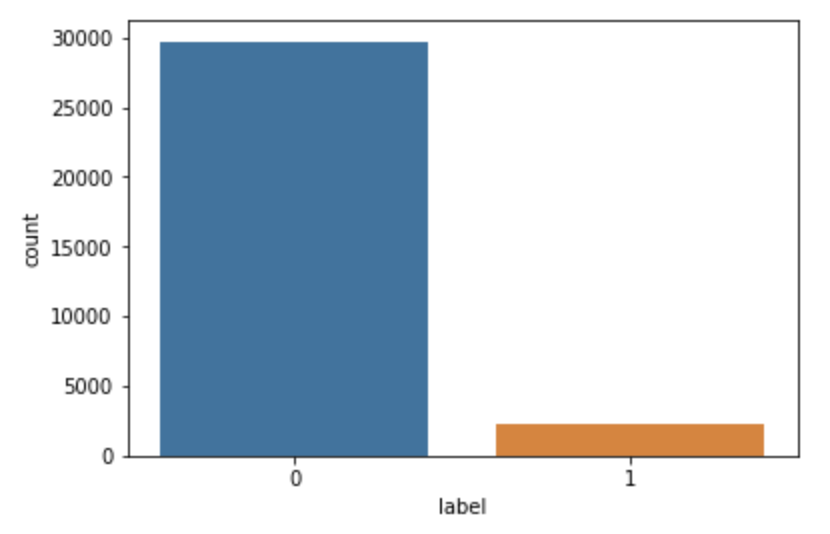
\includegraphics[width=9cm]{classes.png}
		\centering
	\end{figure}
	
	\subsection{Test Set}
	
	The test set is composed by 17197 observations, with only two columns ("id" and "tweet"). Given that this challenge is an open challenge, makes sense no "label" column, to make users submit their results. 
	
	\section{Initial Feature Engineering}
	
	\subsection{Pre-clean Tweet length}
	
	Given that in NLP tasks the most difficult challenge is the feature engineering part, and after applying algorithms out-of-box \textbf{after} cleaning and I was not able to produce good results, I tried to create my own features. 
	
	So the first hypothesis that I wanted to test was if one class of tweets has a statistically different pre-clean length that the other one. As we can see in Figure 2:
	
	\begin{figure}[h]
		\label{Figure 1}
		\caption{Pre-clean length}
		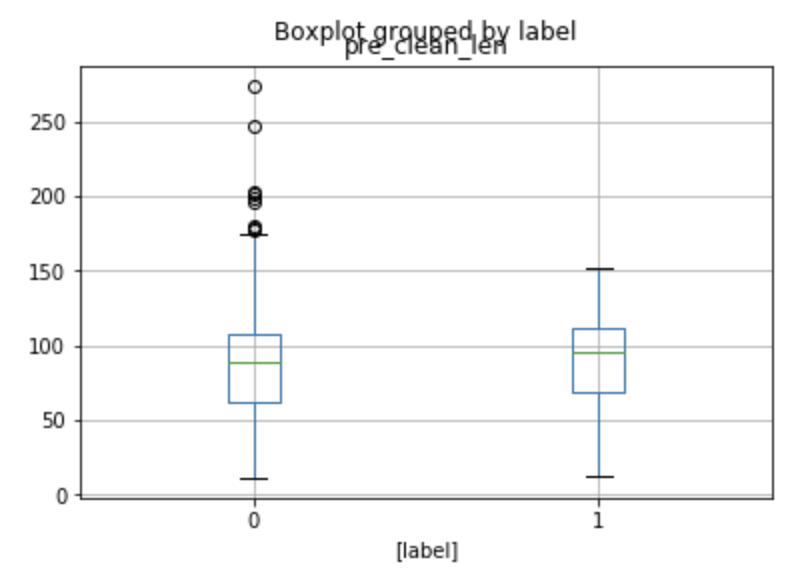
\includegraphics[width=9cm]{precleanl.png}
		\centering
	\end{figure}
	
	So, in terms of the median value, there is not a significant difference, but the $75^{th}$ percentile is somewhat deviated in class 0, comparing to class 1.  
	
	\subsection{Number of exclamation marks}
	
	So following the same line of thought of the last subsection, I thought that exclamation marks could be a discriminative feature. The hypothesis was that hate-speech tweets had more exclamation marks than non-hate speech tweets. The boxplot for each class in terms of the number of number of exclamation points. 
	
	\begin{figure}[h]
		\label{Figure 2}
		\caption{Number of Exclamation Marks}
		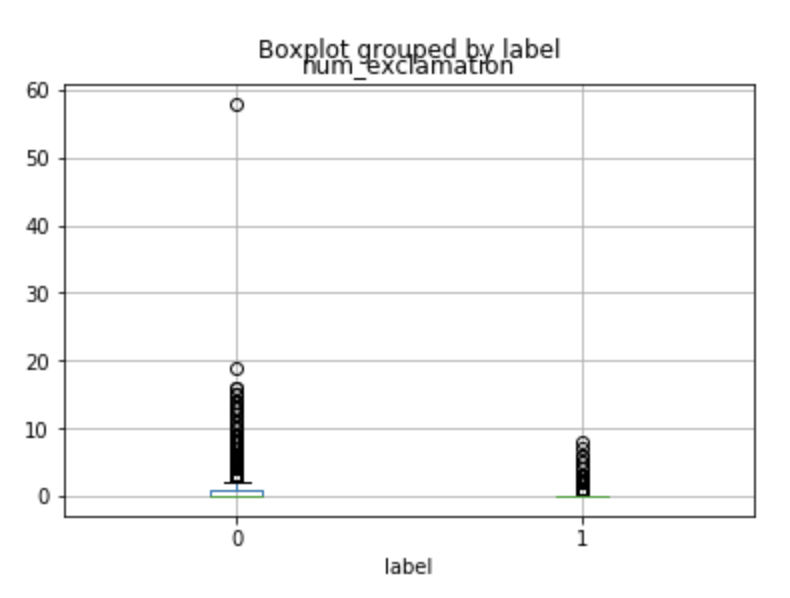
\includegraphics[width=9cm]{postcleanlength.png}
		\centering
	\end{figure}
	
	Again, there is not a significant difference between the two, but we can see, opposite to what I thought could be possible, the non-hate speech class has more exclamation marks. 
		
	\subsection{Post-cleaning length}
	
	Skipping some steps, lets now check the post-cleaning length. Again, there is no statistically  significant differences between one class and the other. This can be seen in Figure 4. 
	
	\begin{figure}[h]
		\label{Figure 3}
		\caption{Post-cleaning length}
		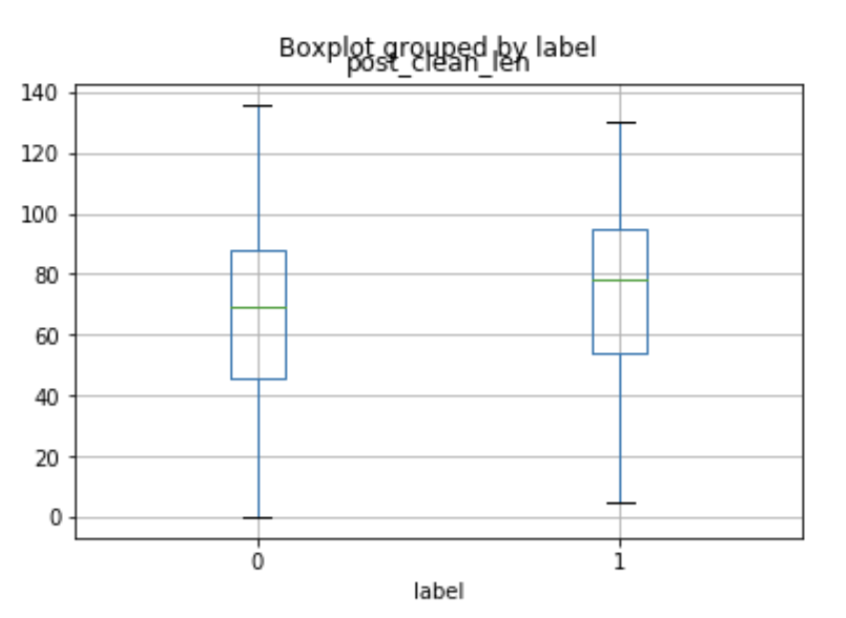
\includegraphics[width=9cm]{post.png}
		\centering
	\end{figure}

	\section{Data Cleaning}
	
	In this section, I will refer the cleaning steps that I took.
	
	Given that the dataset already had user mentions anonymised, these mentions, in my opinion, did not had any predictive power. Given this, I wrote a function, called \texttt{remove\_pattern(text, pattern)} that can remove any pattern of a \textit{regex} expression. I applied this function to the data set column \texttt{tweet}, creating a new column, named \texttt{new\_tweet}.
	
	The second step of the cleaning part was to lowercase each word of the column. This operation was applied to the \texttt{new\_tweet} column. 
	
	The cleaning part of this project was also accomplished using another function \texttt{clean\_tweet(text)}, that perform the following steps:
	\begin{itemize}
		\item Remove HTML characters.
		\item Encoding normalization.
		\item Check for common abbreviation in english and transform them to the long version (like "aren't" to "are not").
		\item Remove non-character symbols.
		\item Tokenize each tweet using the NLTK Tokenizer.
	\end{itemize}
	
	Then checked for missing values in all columns, that produced no results. 
	
	\section{Exploratory Data Analysis}
	
	\subsection{Word Cloud}
	
	For the positive class (non-hate speech), this is the word clouds after removing the stop words (Figure 5).
	
	\begin{figure}[h]
		\label{Figure 5}
		\caption{WordCloud for non-hate speech class}
		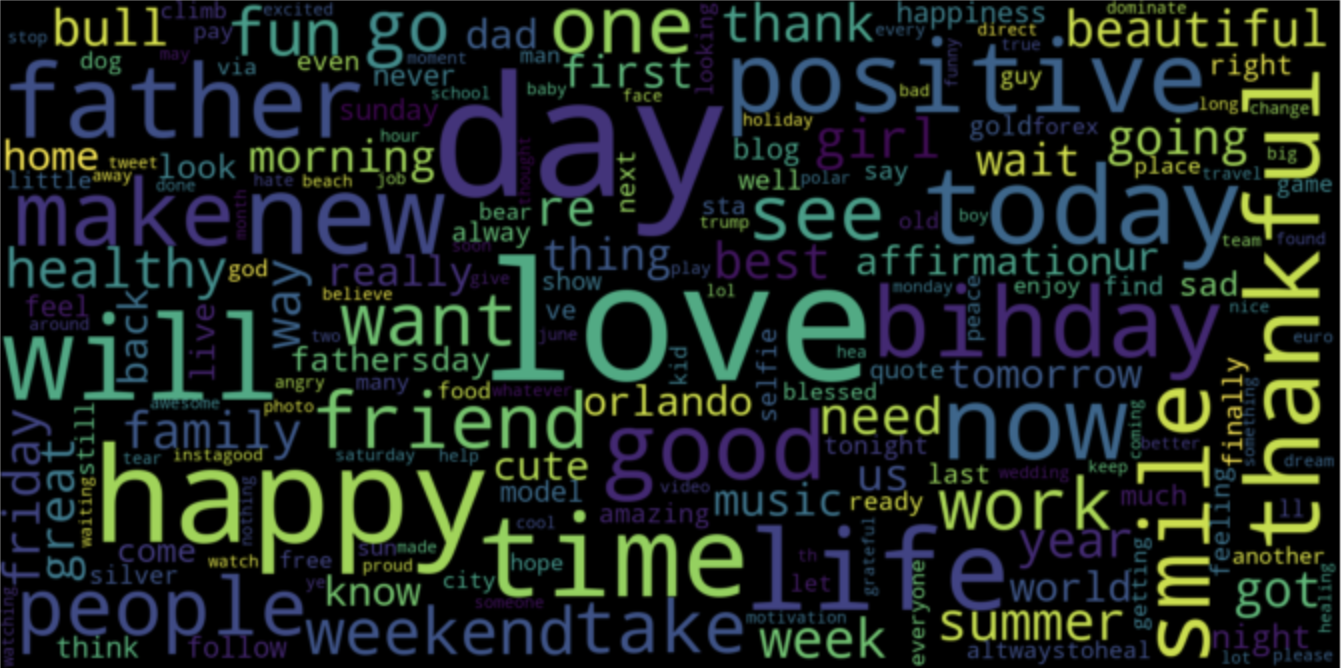
\includegraphics[width=9cm]{wordpos.png}
		\centering
	\end{figure}
	
	Now for the negative class (hate speech tweets), the word cloud can be seen in Figure 6.
	
	\begin{figure}[h]
		\label{Figure 6}
		\caption{WordCloud for hate speech class}
		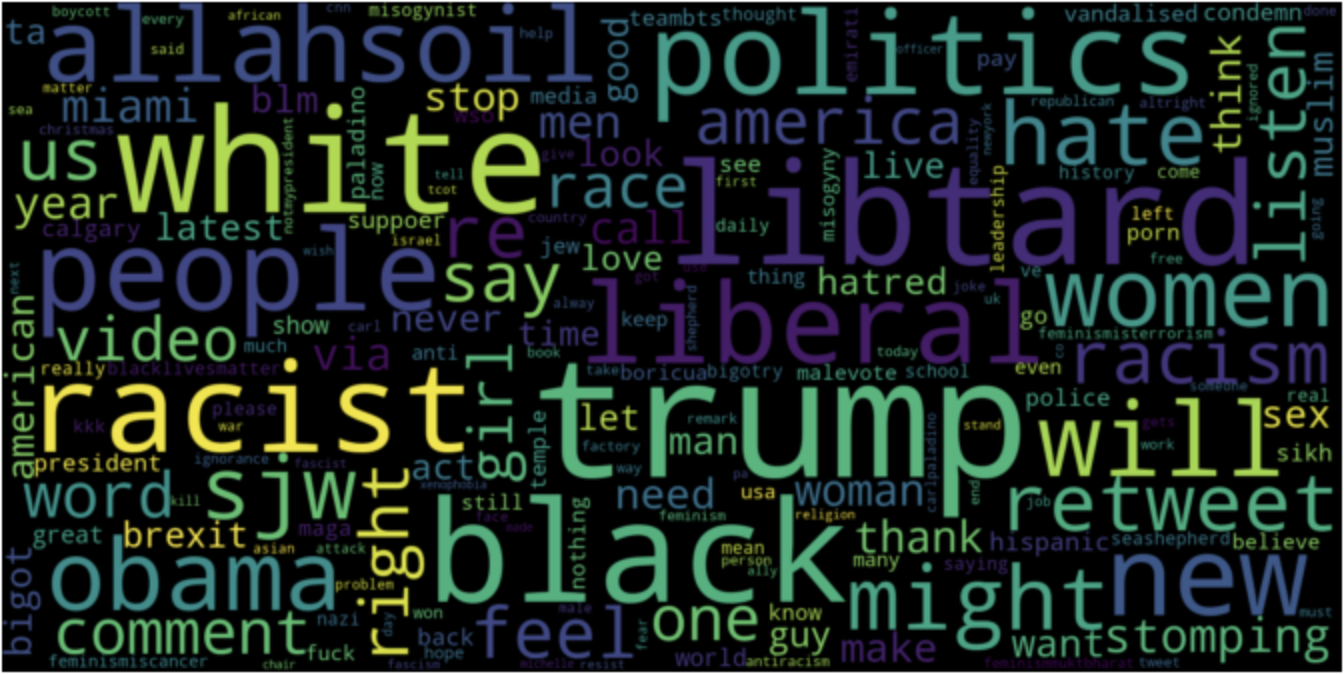
\includegraphics[width=9cm]{wordneg.png}
		\centering
	\end{figure}
	
	\subsection{Zipf's Law}
	
	Zipf’s Law states that a small number of words are used all the time, while the vast majority are used very rarely. There is nothing surprising about this, we know that we use some of the words very frequently, such as “the”, “of”, etc, and we rarely use the words like “aardvark” (aardvark is an animal species native to Africa). However, what’s interesting is that “given some corpus of natural language utterances, the frequency of any word is inversely proportional to its rank in the frequency table. Thus the most frequent word will occur approximately twice as often as the second most frequent word, three times as often as the third most frequent word, etc.”
	
	\begin{figure}[h]
		\label{Figure 7}
		\caption{Approximate Zipf Law}
		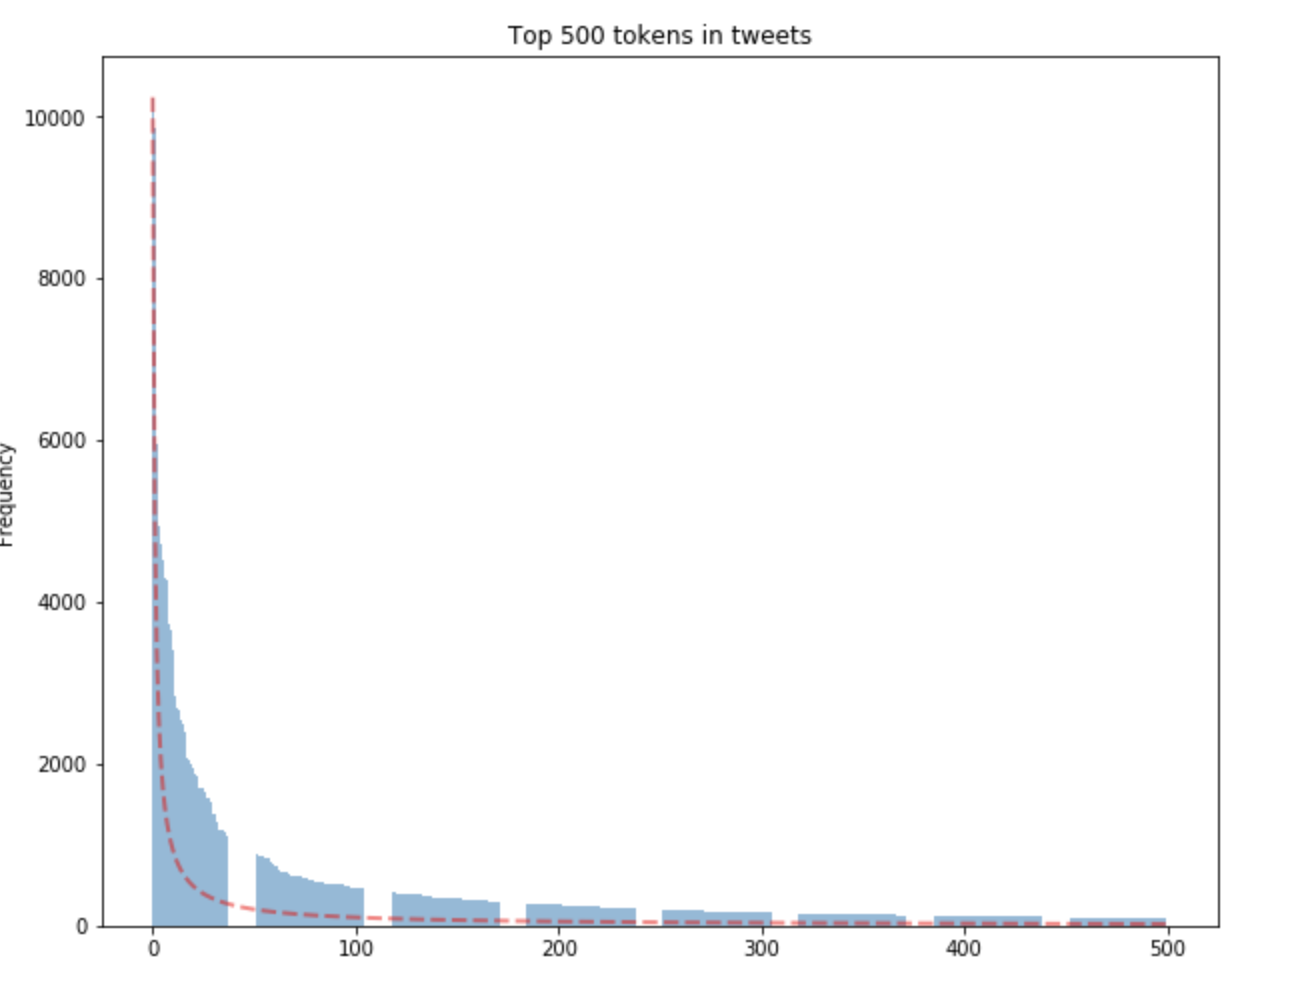
\includegraphics[width=9cm]{zipf.png}
		\centering
	\end{figure}
	
	
	In Figure 7, the x-axis is the rank of the frequency from highest rank from left up to 500th rank to the right. Y-axis is the frequency observed in the corpus (in this case, our dataset). One thing to note is that the actual observations in most cases does not strictly follow Zipf’s distribution, but rather follow a trend of “near-Zipfian” distribution.
	
	Another way to look at this data is to plot the features at a log-scale. This can be seen in Figure 8.
	
	\begin{figure}[h]
		\label{Figure 8}
		\caption{Log-scaled approximate Zipf Law}
		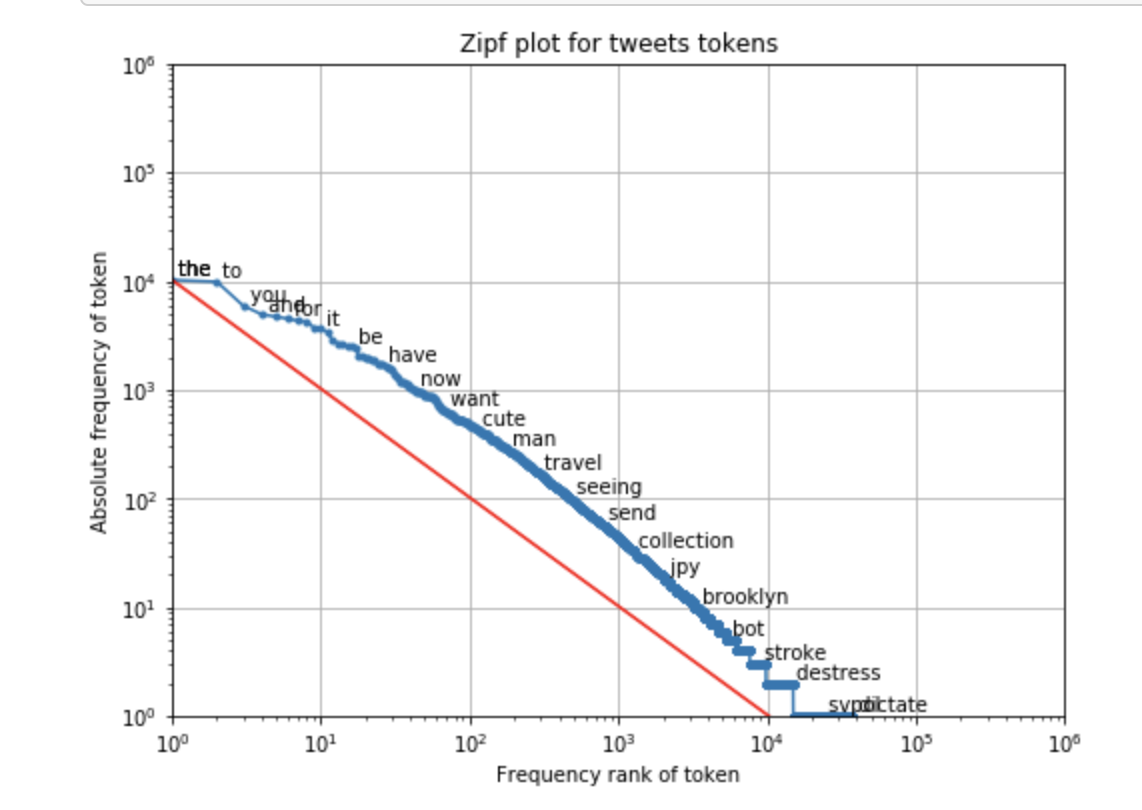
\includegraphics[width=9cm]{logzipf.png}
		\centering
	\end{figure}
	
	\subsection{Token Frequency}
	
	Now let's go deeper into token frequency and test several metrics in order to see if we can extract meaningful information from this set of metrics.
	
	\paragraph{Token count per class}
	
	After removing the stop words, the first question was "how many times a certain token appears in one class?". 
	But lets look at the frequency values of the minority class. Everything is pretty normal, right? (In terms of the ratio between the positives and negatives). What about words like "like", "just"? (Figure 9). 
	
	\begin{figure}[h]
		\label{Figure 9}
		\caption{Token frequency per class}
		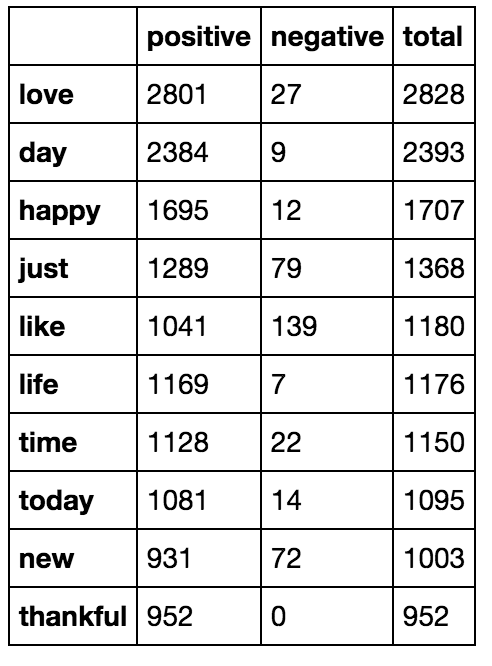
\includegraphics[scale=0.5]{freq1.png}
		\centering
	\end{figure}
	
	\paragraph{Most common tokens per class}
	
	So I started to look for the most common tokens after removing the stop words. In Figure 10 and Figure 11, this can be seen. 
		
	\begin{figure}[h]
		\label{Figure 10}
		\caption{Token frequency per class}
		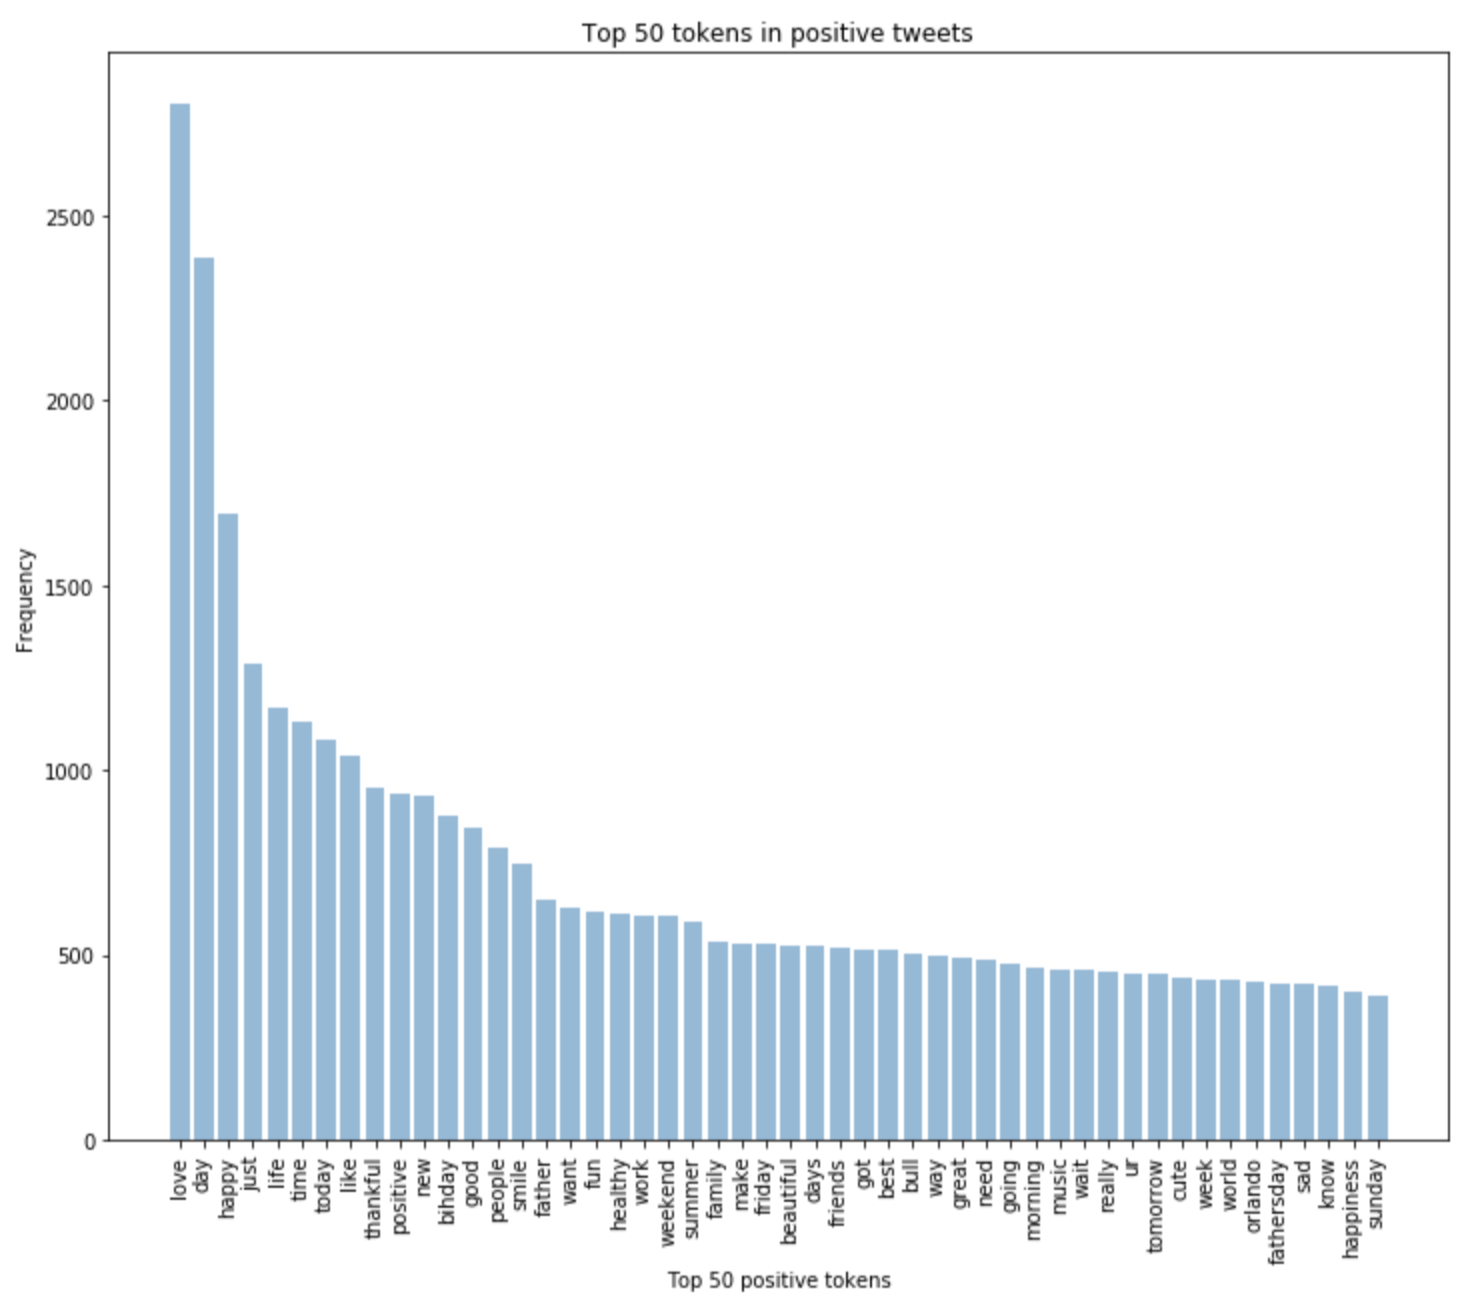
\includegraphics[scale=0.3]{posfreq.png}
		\centering
	\end{figure}
	
			
	\begin{figure}[h]
		\label{Figure 11}
		\caption{Token frequency per class}
		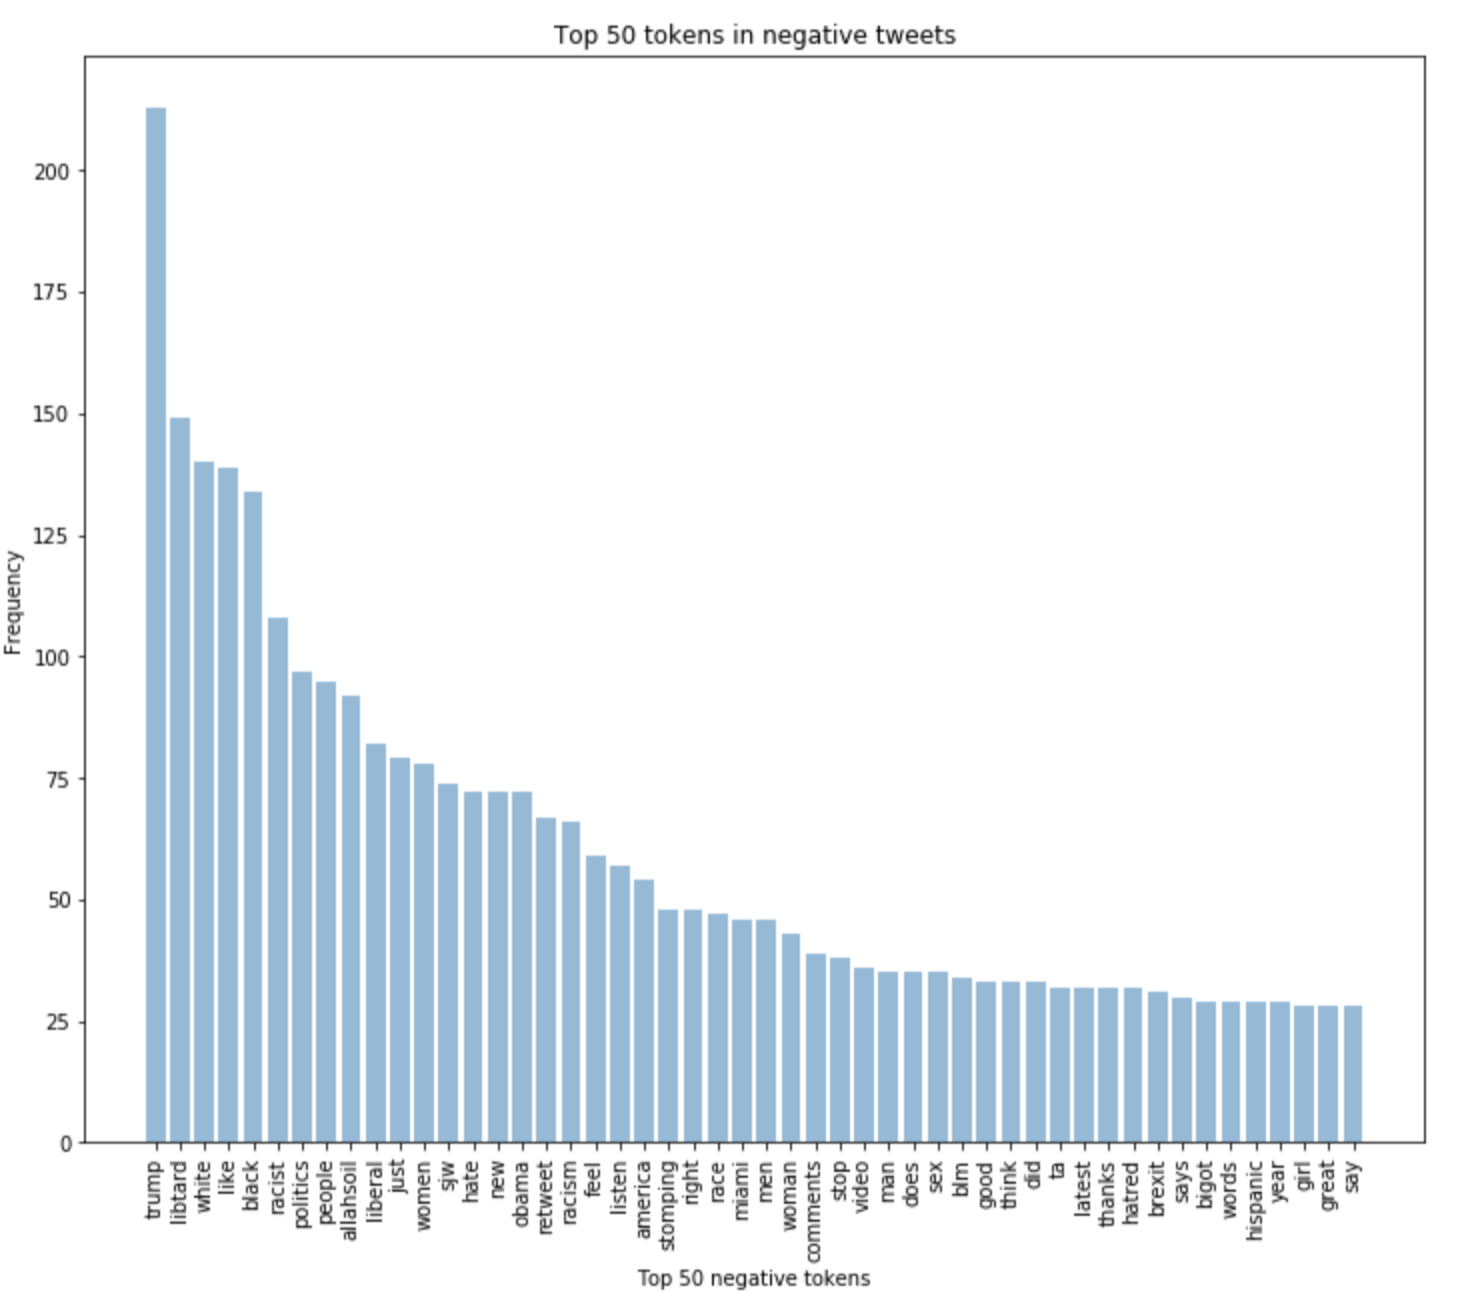
\includegraphics[scale=0.3]{negfreq.png}
		\centering
	\end{figure}
	
	After this, I tried to plot the frequency of the positive and negative tokens in a scatter plot (Figure 12):
	
	\begin{figure}[h]
		\label{Figure 12}
		\caption{Token frequency per class}
		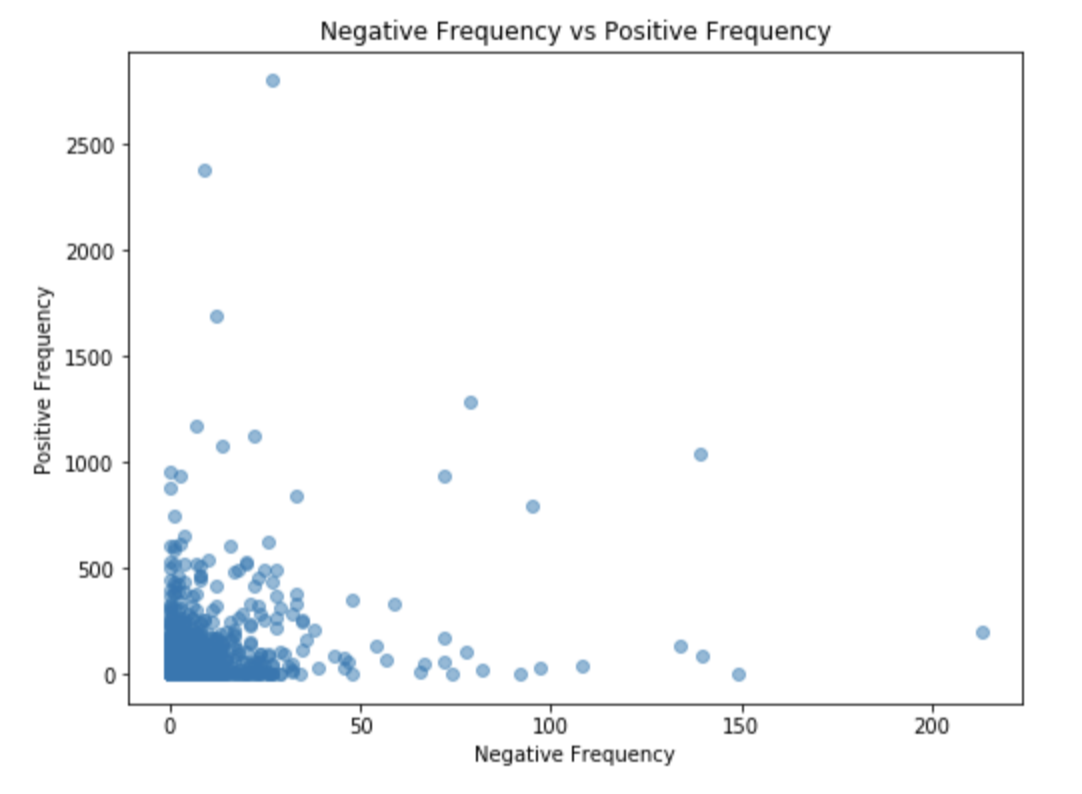
\includegraphics[scale=0.55]{neg_post_freq.png}
		\centering
	\end{figure}

	In the plot above, my goal was to find if there is some relationship between the frequency in relation to positive and negative tokens. The scale of the plot is not the same in the two axis, so one has to be careful when analyzing this results.

NOTE: each point represents a token!

NOTE 2: The tokens that are more meaningful are the ones in the 1st and 4th quarter. The point of no significant would be the points in the line y=x. A measure of meaningfulness would be the distance to this line!

\paragraph{Other Metrics}


Using the metrics for ranking tokens from this \url{https://www.youtube.com/watch?v=H7X9CA2pWKo} PyData Conference, let’s explore what we can get out of frequency of each token. Intuitively, if a word appears more often in one class compared to another, this can be a good measure of how much the word is meaningful to characterise the class.

I call this the \texttt{pos\_rate}, that basically is a measure of how much a token appears in the positive class related to the positive and negative classes.

So the metric above is not really useful, because, this rate can be really high if a word appears few times in the positive class and none on the negative class.

Given this, I used other metric, \texttt{pos\_freq\_pct}, that basically measures the frequency in class.

But since \texttt{pos\_freq\_pct} is just the frequency scaled over the total sum of the frequency, the rank of \texttt{pos\_freq\_pct} is exactly same as just the positive frequency.

So, and borrowing again from the metrics used in the PyData Conference in the ScatterText package, I wanted to combine the two metric above. However, the range of the two metric is different. Although they both range in the interval [0, 1] the frequency in-class ranges from [\~0.0072, 0] and the \texttt{pos\_rate} metric from [0,1]. If I computed the average between the two, one of the metric would have much more weight in the final result than the other.

“Since the harmonic mean of a list of numbers tends strongly toward the least elements of the list, it tends (compared to the arithmetic mean) to mitigate the impact of large outliers and aggravate the impact of small ones.”

The harmonic mean rank seems like the same as \texttt{pos\_freq\_pct}. By calculating the harmonic mean, the impact of small value (in this case, \texttt{pos\_freq\_pct}) is too aggravated and ended up dominating the mean value. This is again exactly same as just the frequency value rank and doesn’t provide a much meaningful result.

What we can try next is to get the CDF (Cumulative Distribution Function) (inspiration taken from here: \url{https://svn.spraakdata.gu.se/repos/richard/pub/statnlp2016_web/l3.pdf} value of both \texttt{pos\_rate} and \texttt{pos\_freq\_pct}. CDF can be explained as “distribution function of X, evaluated at x, is the probability that X will take a value less than or equal to x”. By calculating CDF value, we can see where the value of either \texttt{pos\_rate} or \texttt{pos\_freq\_pct} lies in the distribution in terms of cumulative manner.

	\begin{figure}[h]
		\label{Figure 12}
		\caption{Token frequency per class}
		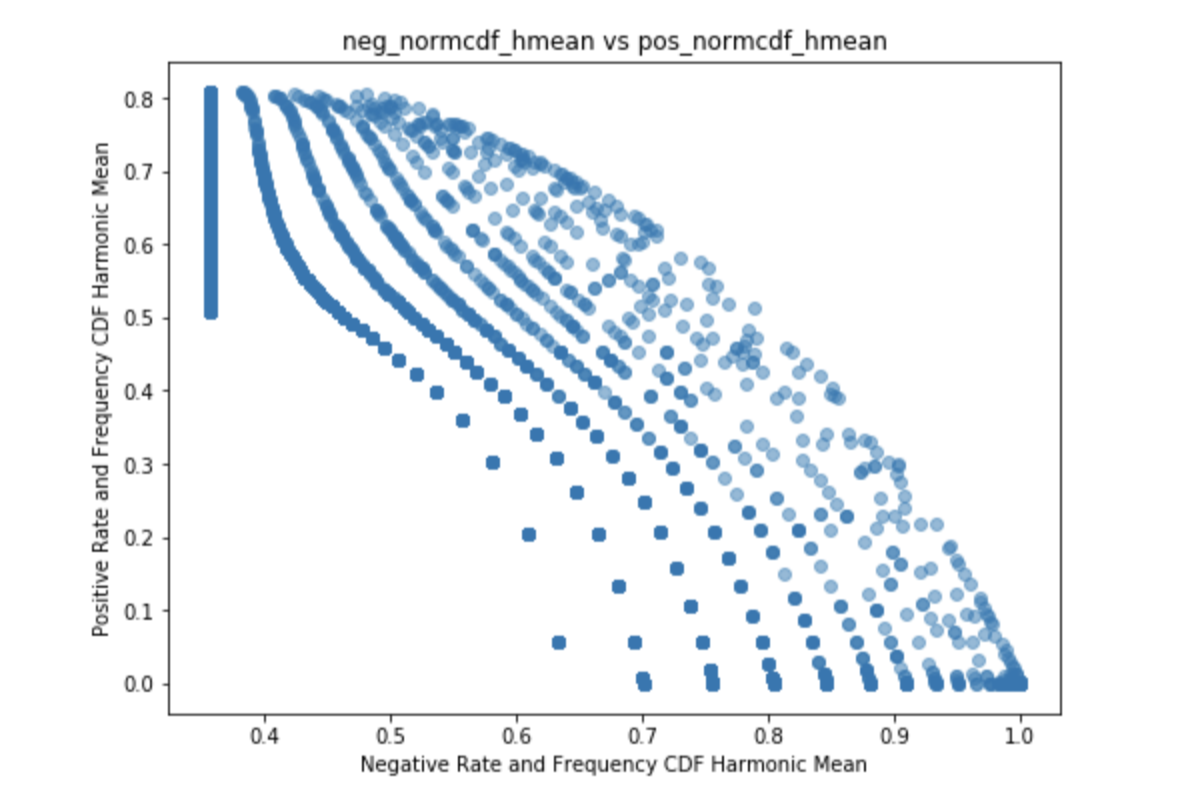
\includegraphics[scale=0.55]{norcdf.png}
		\centering
	\end{figure}


So finally, we can see that there is a relationship between the positive and negative samples. Each data point represents a token, and tokens in the first quarter are the most significant in terms of "positivity", and the data points in the fourth quarter are the most significant in terms of "negativity".


	
	\section{Algorithms \& Feature Engineering}
	\subsection{Logistic Regression}
	
	The first algorithm that I chose, given that I have worked before with logistic regression and due to being a quite interpretable and simple algorithm, I started the algorithmic part using Logistic Regression. In Figure 14, we can check the results using different \texttt{n\_gram} ranges and different number of features extracted using TF-IDF feature extraction mechanism. 
	
	\begin{figure}[h]
		\label{Figure 14}
		\caption{Logistic Regression results}
		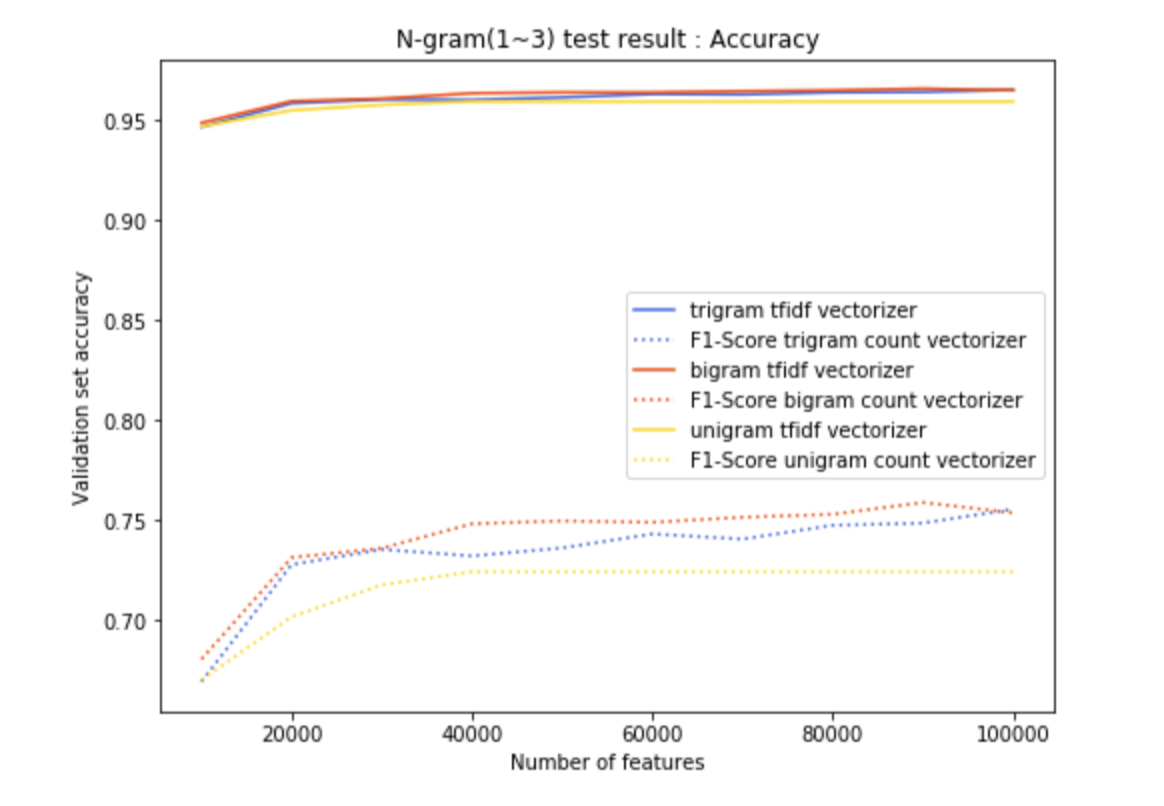
\includegraphics[scale=0.55]{LR.png}
		\centering
	\end{figure}


	\subsection{Algorithm Comparison}
	
	In this subsection, I experimented using different supervised algorithms with the number of features and \texttt{n\_gram} range found to produced the best results when applying the Logistic Regression algorithm. The results can be checked in Table 1. 
	
	% Please add the following required packages to your document preamble:
% \usepackage{graphicx}
\begin{table}[h]
\caption{Algorithm Comparison}
\label{my-label}
\resizebox{\textwidth}{!}{%
\begin{tabular}{lllllll}
\hline
Algorithm & \begin{tabular}[c]{@{}l@{}}Hyperparameters\\ Tuned\end{tabular} & Feature Extraction Mechanism & \begin{tabular}[c]{@{}l@{}}N-Gram\\ Range\end{tabular} & Number of Features & \begin{tabular}[c]{@{}l@{}}Accuracy\\ (Validation Set)\end{tabular} & \begin{tabular}[c]{@{}l@{}}F1-Score\\ (Validation Set)\end{tabular} \\ \hline
LR & Yes & TF-IDF & 1,2 & 90000 & 96.18\% & 75.88\% \\ \hline
LinearSVC & Yes & TF-IDF & 1,2 & 90000 & 96.32\% & 69.99\% \\ \hline
LinearSVC with L1 FS & Yes & TF-IDF & 1,2 & 90000 & 94.89\% & 66.53\% \\ \hline
AdaBoostClassifier & Yes & TF-IDF & 1,2 & 90000 & 94.82\% & 50.08\% \\ \hline
MultinomialNB & No & TF-IDF & 1,2 & 90000 & 94.31\% & 30.00\% \\ \hline
BernoulliNB & No & TF-IDF & 1,2 & 90000 & 94.27\% & 29.62\% \\ \hline
RidgeClassifier & Yes & TF-IDF & 1,2 & 90000 & 35.32\% & 11.66\% \\ \hline
PassiveAggressiveClassifier & Yes & TF-IDF & 1,2 & 90000 & 92.63\% & 51.73\% \\ \hline
Perceptron & Yes & TF-IDF & 1,2 & 90000 & 95.42\% & 60.12\% \\ \hline
NearestCentroid & No & TF-IDF & 1,2 & 90000 & 96.03\% & 70.12\% \\ \hline
\end{tabular}%
}
\end{table}

\paragraph{Doc2Vec}

In this part of this report, I will go through the experiments that I did using a different kind of feature extraction mechanism, called Doc2Vec. Given that this method learns a probabilistic (versus frequentist, like TF-IDF) vectorized representation of words, and this learning part is of unsupervised nature, the test data was used in this part. In Table 2, the results of different techniques can be observed and compared. 

% Please add the following required packages to your document preamble:
% \usepackage{graphicx}
\begin{table}[]
\caption{Doc2Vec Results}
\label{my-label}
\resizebox{\textwidth}{!}{%
\begin{tabular}{llll}
\hline
Algorithm & Doc2Vec Technique & \begin{tabular}[c]{@{}l@{}}Accuracy\\ (Validation Set)\end{tabular} & \begin{tabular}[c]{@{}l@{}}F1-Score\\ (Validation Set)\end{tabular} \\ \hline
Logistic Regression & DBOW & 80.15\% & 35.87\% \\ \hline
Logistic Regression & DMC & 86.01\% & 29.08\% \\ \hline
Logistic Regression & DMC+DBOW & 91.53\% & 35.84\% \\ \hline
\end{tabular}%
}
\end{table}

	\subsection{Deep Learning}

	The results when using various deep learning models can be seen in Table 3. 
	
	% Please add the following required packages to your document preamble:
% \usepackage{graphicx}
% Please add the following required packages to your document preamble:
% \usepackage{graphicx}
\begin{table}[h]
\caption{Deep Learning results}
\label{my-label}
\resizebox{\textwidth}{!}{%
\begin{tabular}{llllllllllll}
\hline
Type & \begin{tabular}[c]{@{}l@{}}Number of\\ Layers\end{tabular} & \begin{tabular}[c]{@{}l@{}}Size of \\ Layers\end{tabular} & Epochs & Batch Size & Batch Shuffle & \begin{tabular}[c]{@{}l@{}}Batch\\ Normalization\end{tabular} & Optimizer & Dropout & Features & \begin{tabular}[c]{@{}l@{}}Accuracy \\ (Validation Set)\end{tabular} & \begin{tabular}[c]{@{}l@{}}F1-Score\\ (Validation Set)\end{tabular} \\ \hline
MLP & 1 & 64 & 10 & 256 & No & No & ADAM & No & TF-IDF & 95.39\% & 67.05\% \\ \hline
MLP & 2 & 128/64 & 10 & 256 & No & No & ADAM & No & TF-IDF & 95.71\% & 65.91\% \\ \hline
MLP & 1 & 64 & 10 & 32 & Yes & No & ADAM & No & TF-IDF & 95.10\% & 4.86\% \\ \hline
MLP & 1 & 64 & 10 & 32 & No & Yes & ADAM & No & TF-IDF & 95.12\% & 4.86\% \\ \hline
MLP & 1 & 64 & 10 & 32 & Yes & Yes & ADAM & Yes / 0.2 & TF-IDF & 95.18\% & 4.61\% \\ \hline
MLP & 1 & 64 & 10 & 32 & Yes & Yes & \begin{tabular}[c]{@{}l@{}}Custom ADAM\\ Lr=0.005\end{tabular} & No & TF-IDF & 94.92\% & 4.77\% \\ \hline
MLP & 1 & 64 & 10 & 32 & Yes & Yes & \begin{tabular}[c]{@{}l@{}}Custom ADAM\\ Lr=0.01\end{tabular} & No & TF-IDF & 95.01\% & 4.54\% \\ \hline
MLP & 2 & 128/64 & 40 & 256 & No & No & ADAM & No & \begin{tabular}[c]{@{}l@{}}Doc2Vec\\ (DMC+DBOW)\end{tabular} & 92.55\% & 41.47\% \\ \hline
MLP & 2 & 128/64 & 40 & 256 & No & No & ADAM & No & \begin{tabular}[c]{@{}l@{}}Doc2Vec\\ (DMC+DBOW)\end{tabular} & 93.35\% & 65.64\% \\ \hline
MLP + Embeddings & 2 & 256 & 5 & 256 & No & No & ADAM & No & \begin{tabular}[c]{@{}l@{}}Word2Vec\\ (DBOW)\end{tabular} & 95.25\% & 65.14\% \\ \hline
MLP + Embeddings & 3 & 256/256 & 10 & 256 & No & No & ADAM & No & \begin{tabular}[c]{@{}l@{}}Word2Vec\\ (DBOW)\end{tabular} & 96.02\% & 69.95\% \\ \hline
CNN + Embeddings & 8 & N/A & 10 & 512 & No & No & ADAM & Yes / 0.2 & \begin{tabular}[c]{@{}l@{}}Word2Vec\\ (DBOW)\end{tabular} & 96.77\% & 74.88\% \\ \hline
\end{tabular}%
}
\end{table}
	\section{Discussion and Future Work}
\end{document}